\documentclass[a4paper,12pt]{jarticle}
\input ./chap01_preamble.tex
\graphicspath{%
  {../text01-img/}%
}
% !TEX root = ./chap01_04.tex
\begin{document}
\section{HTML(自己紹介のホームページ)}
みなさんがブラウザでけんさくしてホームページを表示させました。ホームページはHTML(エイチ ティー エム エル)という言語で書かれています。ブラウザがこれを理解して表示をしてくれています。HTMLはテキストエディタで編集します。ホームページはかんたんに作ることができます。この章では、みなさんも作り方を学び、自分の自己紹介のホームページを作ります。


\bigskip


\bigskip


\bigskip


\bigskip



\begin{figure}[hb]
  \centering
  \begin{minipage}{15.801cm}
    {\upshape
      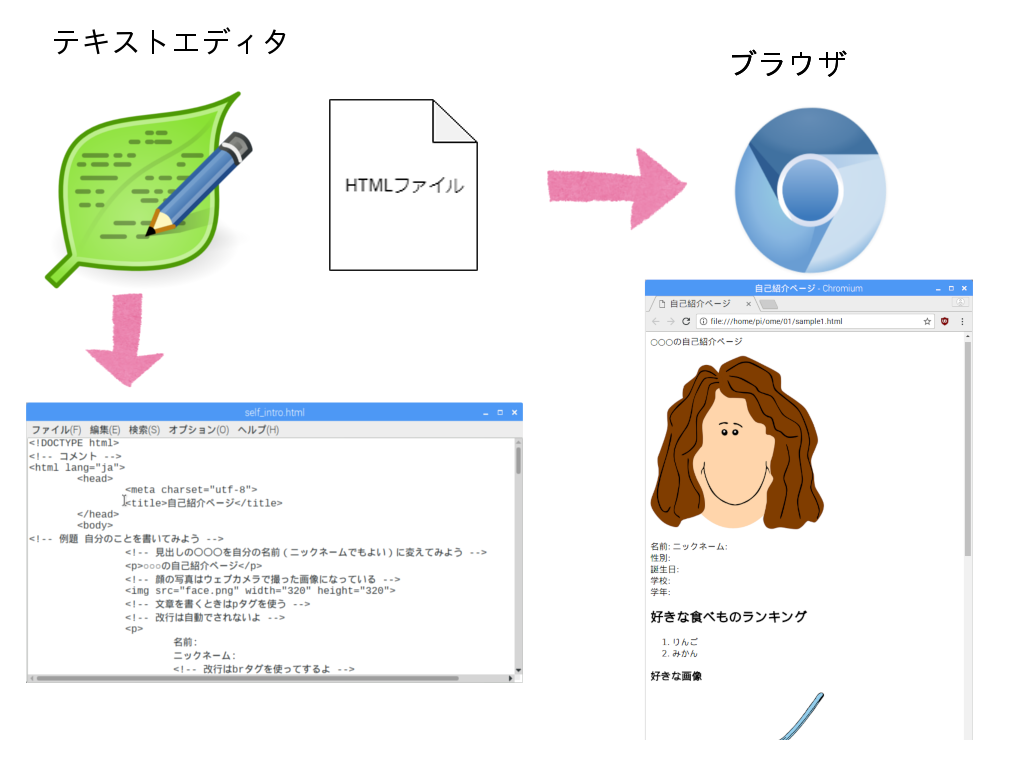
\includegraphics[width=15.801cm]{textbook-img140.png}
      \newline
      \stepcounter{Figure}{\theFigure}: ホームページ作成全体図}
  \end{minipage}
\end{figure}
\clearpage

\begin{figure}
\subsection{教材をじぶんのフォルダに置こう}
ホームページの作り方を学ぶための教材は、/usr/local/share/omeというフォルダに置いてあります。
これを、じぶんのフォルダにコピーしましょう。

\textbf{考え方}

  \bigskip

  \centering
  \begin{minipage}{\textwidth}
    \begin{minipage}{0.45\linewidth}
      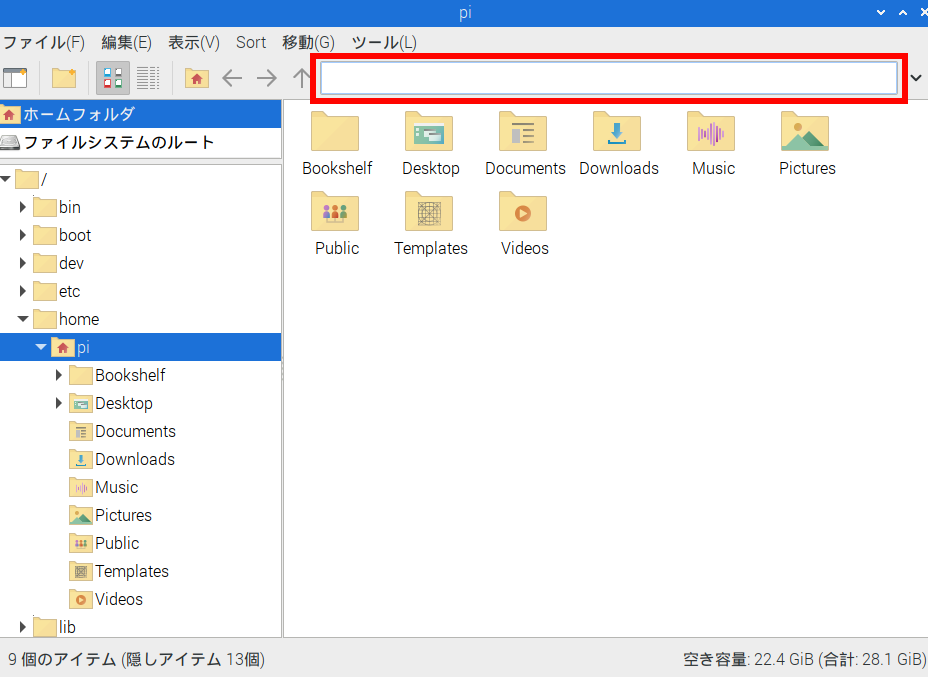
\includegraphics[height=5cm]{textbook-img1010.png}\\
      1.赤い枠で囲ったところをクリックして、/usr/local/share/omeと入力して、エンターキーを押そう
    \end{minipage}
    \hfill
    \vspace{20pt}
    \begin{minipage}{0.45\linewidth}
      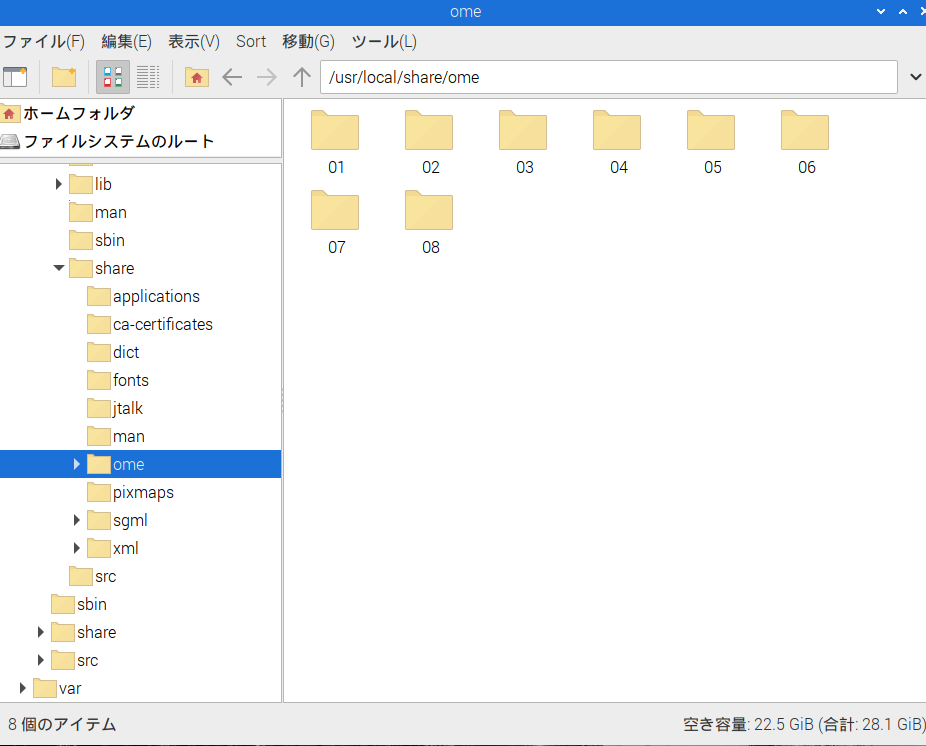
\includegraphics[height=5cm]{textbook-img1011.png}\\
      2.「01」から「08」までのフォルダが表示されていることを確認しよう
    \end{minipage}
    \begin{minipage}{0.45\linewidth}
      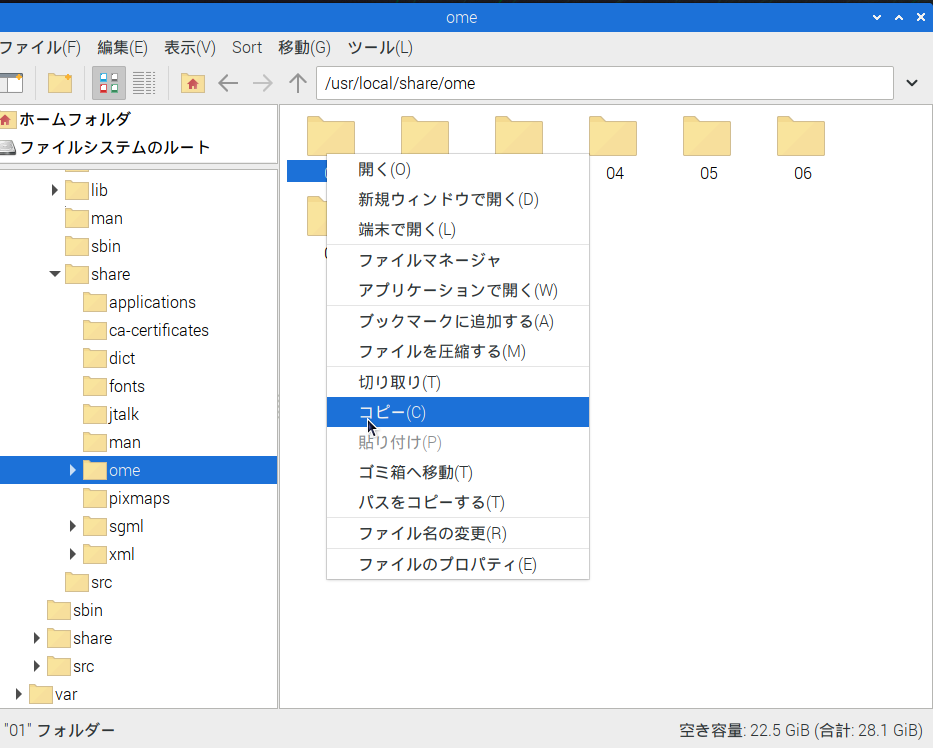
\includegraphics[height=5cm]{textbook-img1012.png}\\
      3.「01」フォルダの上で右クリックし、「コピー」しよう
    \end{minipage}
    \hfill
    \vspace{20pt}
    \begin{minipage}{0.45\linewidth}
      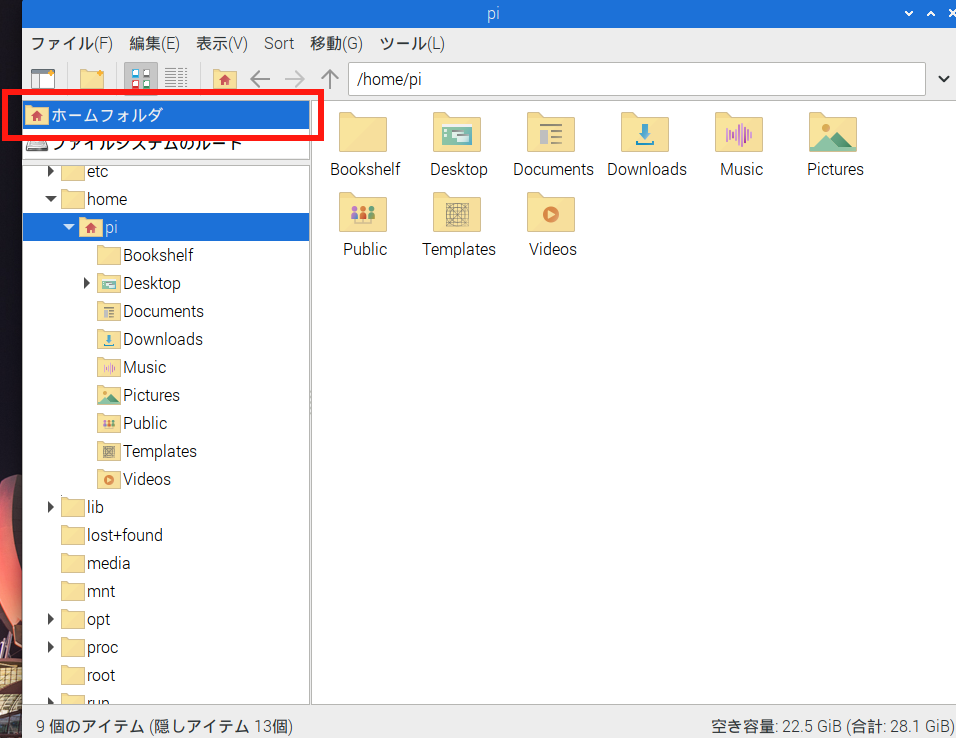
\includegraphics[height=5cm]{textbook-img1013.png}\\
      4.赤い枠で囲った「ホームフォルダ」をクリックして、自分のフォルダに移動しよう
    \end{minipage}    \begin{minipage}{0.45\linewidth}
      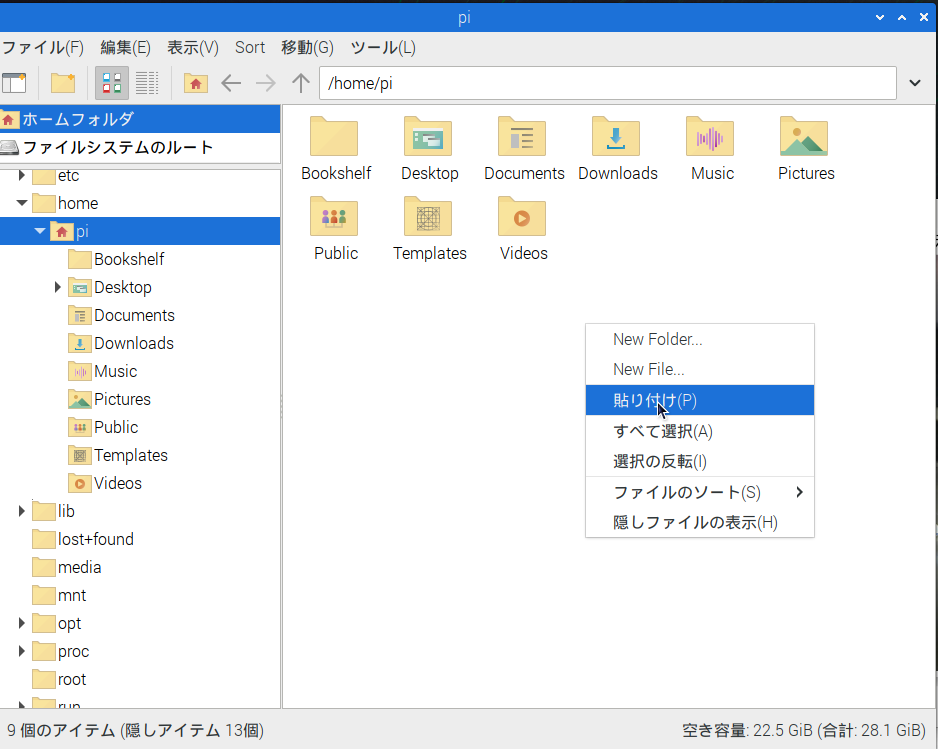
\includegraphics[height=5cm]{textbook-img1014.png}\\
      5.ホームフォルダに移動したら、空いているところをクリックして、さっきコピーしたフォルダを「貼り付け」しよう
    \end{minipage}
    \hfill
    \vspace{20pt}
    \begin{minipage}{0.45\linewidth}
      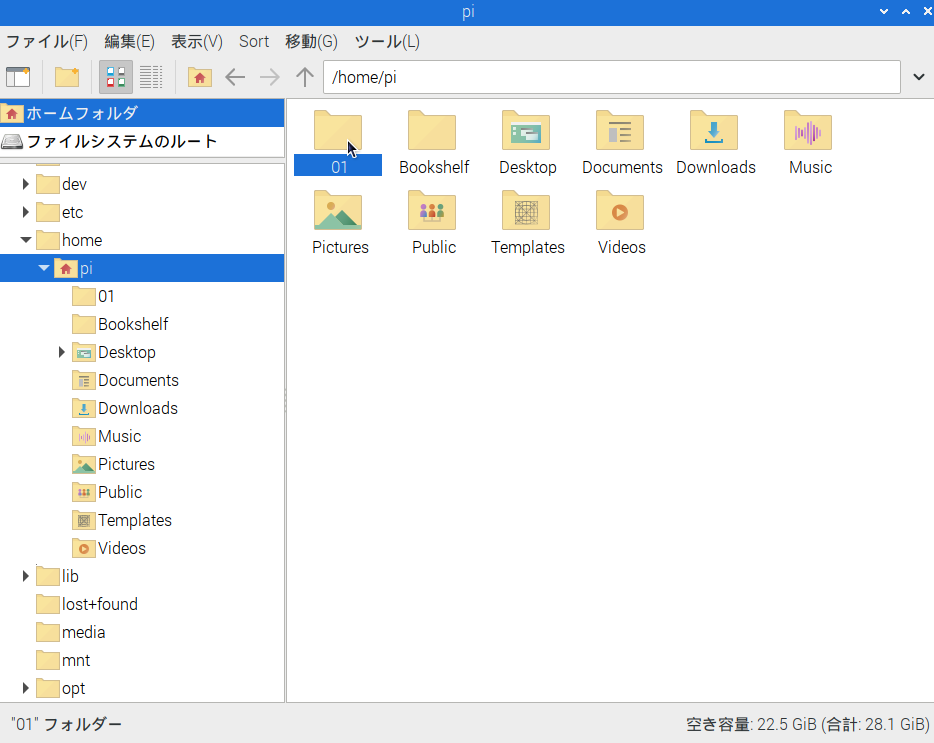
\includegraphics[height=5cm]{textbook-img1015.png}\\
      6.「01」フォルダがあらわれたら、教材のじゅんび完了だよ
    \end{minipage}

  \end{minipage}

  \bigskip

\end{figure}

\bigskip

\clearpage
\refstepcounter{Exercise}
\subsection{\theExercise ホームページの中身を見てみよう}
自己紹介ページのテンプレートを見てみよう

先ほどコピーした01フォルダにあるself\_intro.htmlをブラウザで開いてみよう

\textbf{考え方}



\begin{figure}[hb]
  \centering
  \begin{minipage}{16.576cm}
    さきほどブラウザでけんさくして見たページを\textbf{ホームページ}(正確にはウェブページ)といいます。ホームページを見るにはブラウザを使用しました。ウェブページはファイル名のあとに.html(エイチ
    ティー エム
    エル)とついています。ブラウザはこのhtmlファイルを見ることが目的です。ファイルをダブルクリックすると自動的にブラウザがhtmlファイルを開いてくれます。表示されたホームページを見てみましょう。ファイルマネージャーで01フォルダを開きます。

    赤わくで囲われたところが

    /home\textbf{/自分のユーザ名/01}

    なっていることを確認しておきましょう(この画像の場合だと、ユーザ名がpiなので、/home/pi/01になるよ)

    その中にあるself\_intro.html(黒わくのファイル)をダブルクリックして開きます。




    \bigskip
  \end{minipage}

  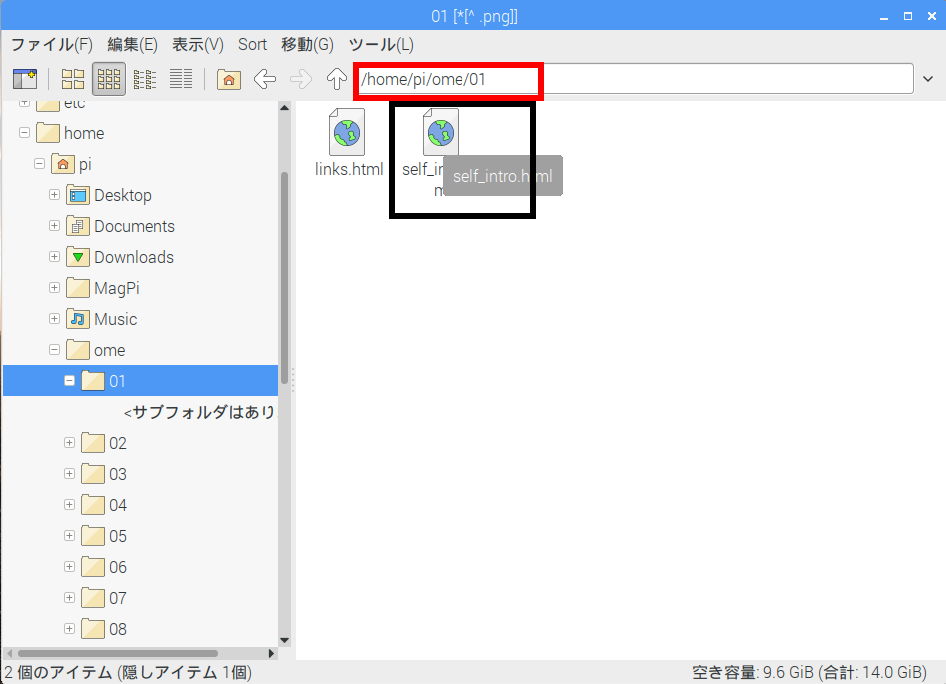
\includegraphics[width=0.8\textwidth]{textbook-img141.png}

\end{figure}

\bigskip

\clearpage
\textbf{答え}



\begin{figure}[hb]
  \centering
  \begin{minipage}{\textwidth}
    このようにホームページが表示されればOKです。

    \centering
    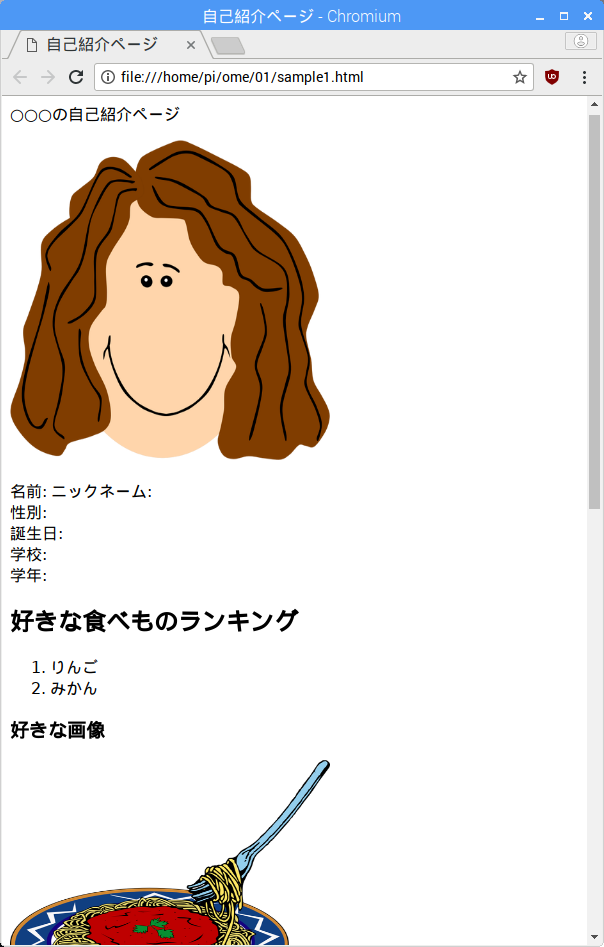
\includegraphics[width=0.4\textwidth]{textbook-img142.png}
  \end{minipage}

\end{figure}
\refstepcounter{Question}\theQuestion\label{Q:hasAnswer04-1}

01フォルダを開いて、links.htmlをブラウザで開いてみよう


\bigskip

\vfill

\clearpage
\begin{figure}[ht]
  \refstepcounter{Exercise}
  \subsection{\theExercise ホームページの中身をのぞいてみよう}
  self\_intro.htmlをテキストエディタで開いて~\ref{seq:refFigure31}のタイトルバーの文字を変更してみよう。タイトルバーは~\ref{seq:refFigure31}のように赤わくで囲われています。


  \bigskip



  \centering
  \begin{minipage}{\textwidth}
    {\upshape
      %\newline
      {\refstepcounter{Figure}\theFigure\label{seq:refFigure31}}:
      ブラウザタイトルバー}
  \end{minipage}

  \centering
  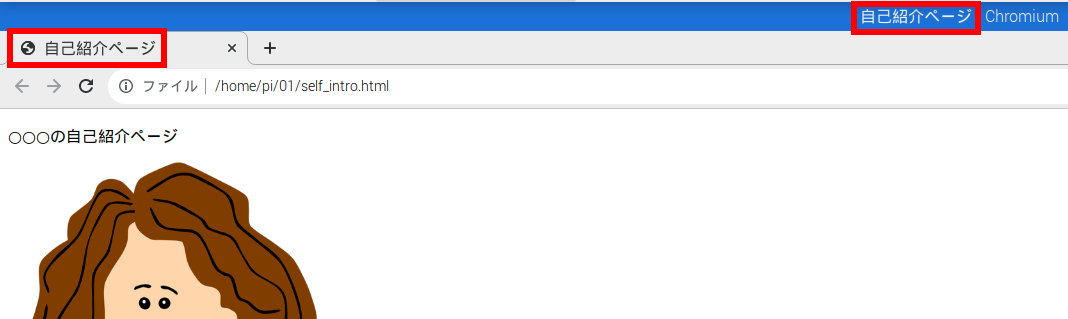
\includegraphics[width=\textwidth]{textbook-img143.png}
  \flushleft
  \textbf{考え方}

  \begin{minipage}{\textwidth}
    \flushleft
    まずは、Text
    Editorでself\_intro.htmlを開いてみましょう。
    \begin{minipage}{0.45\linewidth}
      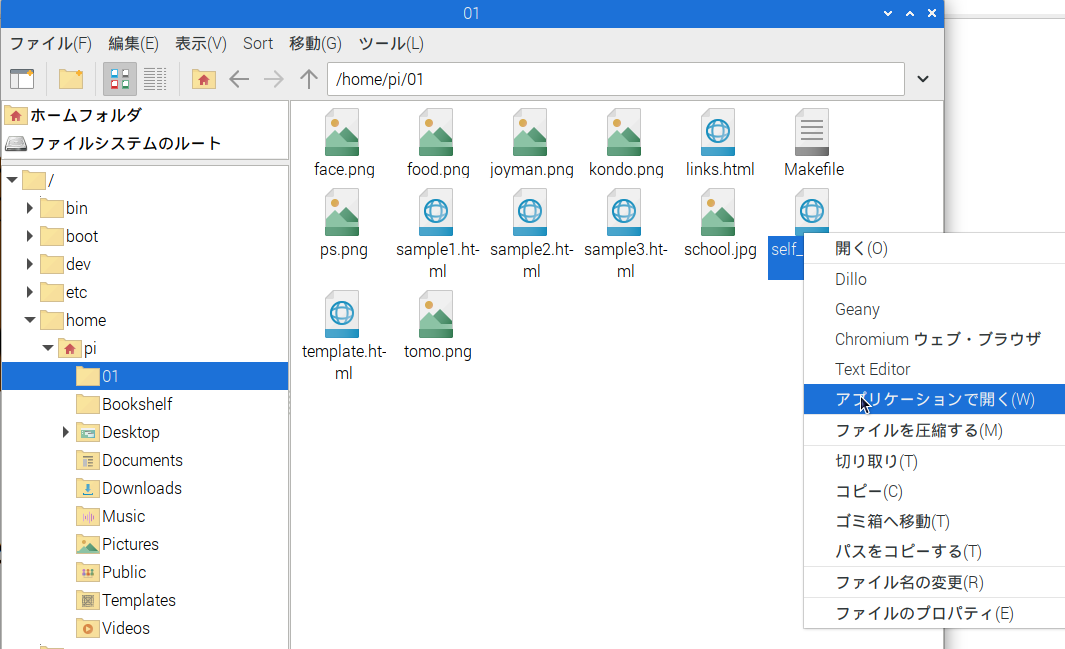
\includegraphics[width=\linewidth]{textbook-img1040.png}\\
      1.self\_intro.htmlを右クリックして、「アプリケーションで開く」をクリックします。
    \end{minipage}
    \hfill
    \vspace{20pt}
    \begin{minipage}{0.45\linewidth}
      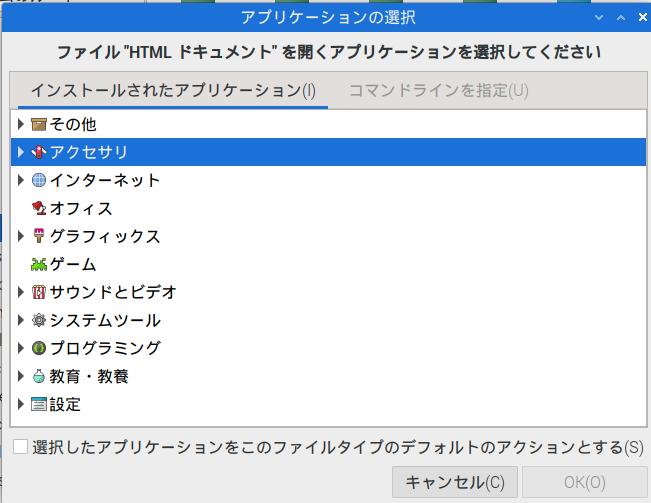
\includegraphics[width=\linewidth]{textbook-img1041.png}\\
      2.「アプリケーションの選択」ウィンドウがでるので、「アクセサリ」をダブルクリックします。
    \end{minipage}
    \begin{minipage}{0.45\linewidth}
      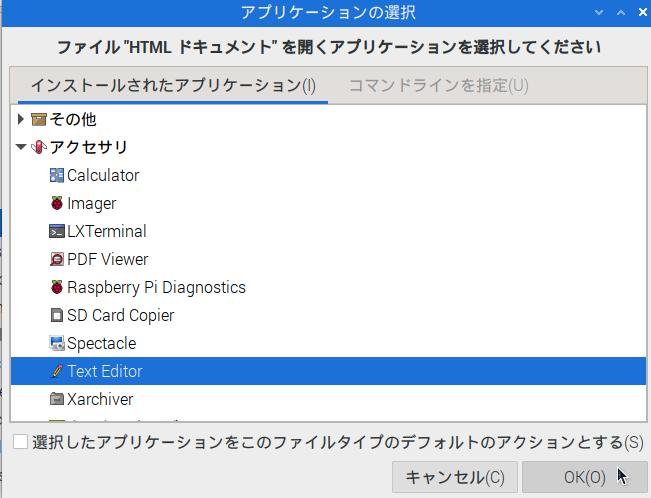
\includegraphics[width=\linewidth]{textbook-img1042.png}\\
      3.「Text Editor」を選んで、OKをクリックします。
    \end{minipage}
  \end{minipage}


\end{figure}

\clearpage
\textbf{考え方(続き)}

Text Editorで開いたら赤線が引かれた
{\textless}title{\textgreater}\textbf{自己紹介ページ}{\textless}/title{\textgreater}
を見てみましょう。\textbf{自己紹介ページ}を変更してみましょう。
この例では\textbf{青梅太郎の自己紹介ページ}と変更します。青梅太郎は自分の名前に置き換えてください。


\centering
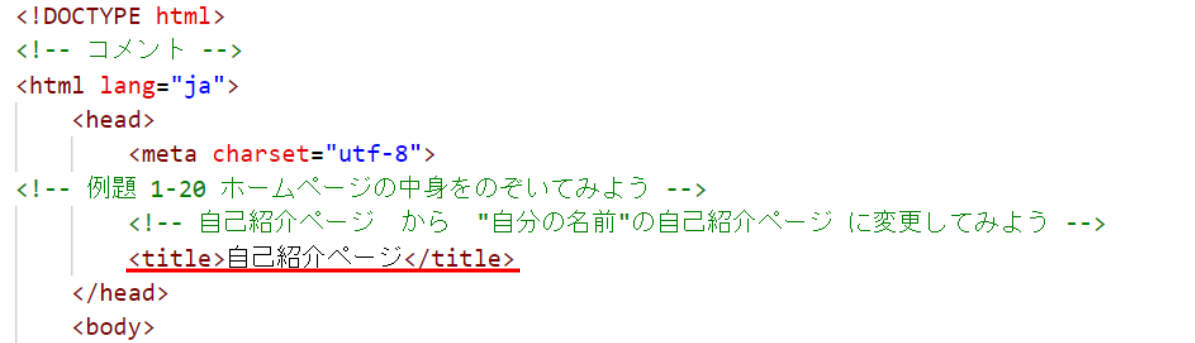
\includegraphics[width=0.9\textwidth]{textbook-img146.png}



\bigskip

\flushleft
変更した例です。

\centering
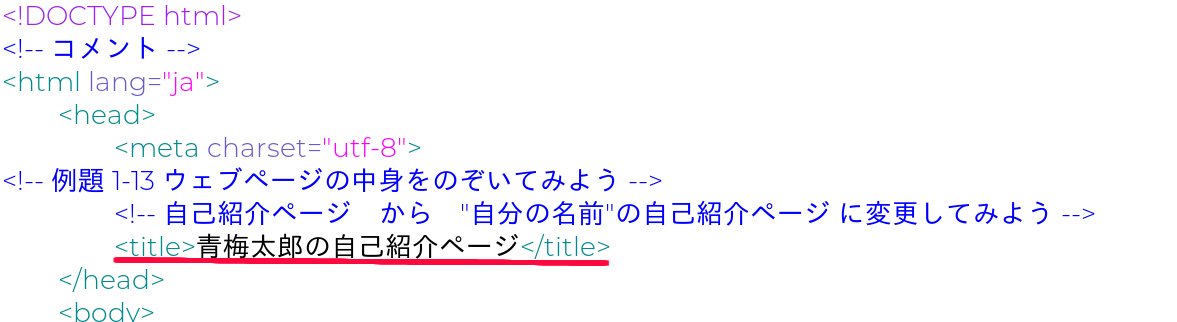
\includegraphics[width=0.9\textwidth]{textbook-img148.png}


\bigskip

\flushleft
変更ができたら、ファイルを保存します。もう一度ファイルの保存の手順を確認しておきます。

ファイルー>保存でファイルを保存することができます。



\centering
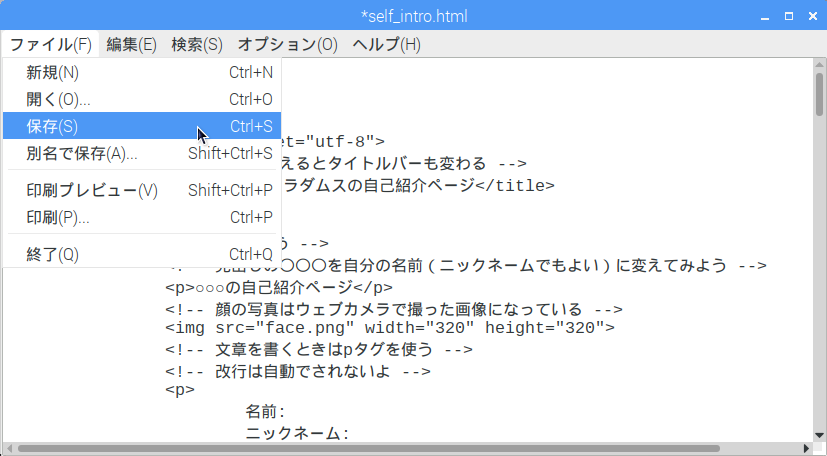
\includegraphics[width=0.8\textwidth]{textbook-img147.png}



\clearpage
\flushleft
\textbf{考え方(続き)}




ファイルに変更をして保存をしました。
変更を見るためには、ブラウザで新しく保存したファイルを読み直す必要があります。
ブラウザでページを読み直すことをリロードといいます。


\bigskip


\bigskip
\centering
%[Warning: Image ignored] % Unhandled or unsupported graphics:
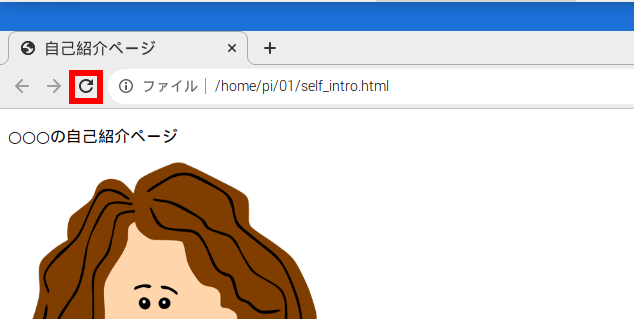
\includegraphics[width=0.8\textwidth]{textbook-img149.png}

\flushleft
赤わくで囲われたように、円の形をした矢印があります。これをクリックすることでリロードができます。これで、変更結果がブラウザへ反映されます。

\vfill
\clearpage
\textbf{答え}


{\textless}title{\textgreater}\textbf{青梅太郎の自己紹介ページ}{\textless}/title{\textgreater}\\
と変更をしたのでブラウザのタイトルバー(赤わくで囲われた部分)はこれに対応して\textbf{青梅太郎の自己紹介ページ}と変わっていますね。

皆さんは、自分の名前が表示されていると思います。

\centering
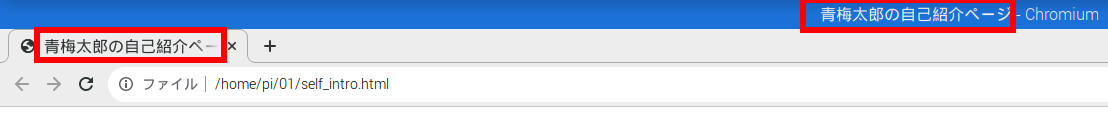
\includegraphics[width=0.85\textwidth]{textbook-img152.png}
\flushleft


二行目に注目してください。

\centering
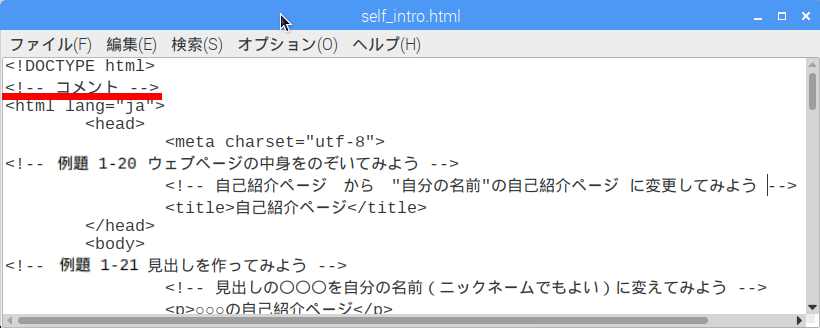
\includegraphics[width=0.85\textwidth]{textbook-img151.png}
\flushleft



\bigskip

{\textless}!- -コメント -
-{\textgreater} という行があります。

これをコメントよびます。囲われたものはブラウザには表示されません。

コメントはメモとして使えます。はじめの{\textless}!-{}-と終わりの{}-{}-{\textgreater}にはスペースは入れてはいけません。この記号の間であれば改行をしても構いません。試しにメモを追加してみましょう。

変えた行の上に

\textbf{ここを変えるとタイトルバーも変わる
}

と追加しましょう。このファイルにはコメントがたくさん書いてあります。変更する前に読んでみてください。コメントはなるべく書いてわかりやすくしておきましょう。


\centering
%[Warning: Image ignored] % Unhandled or unsupported graphics:
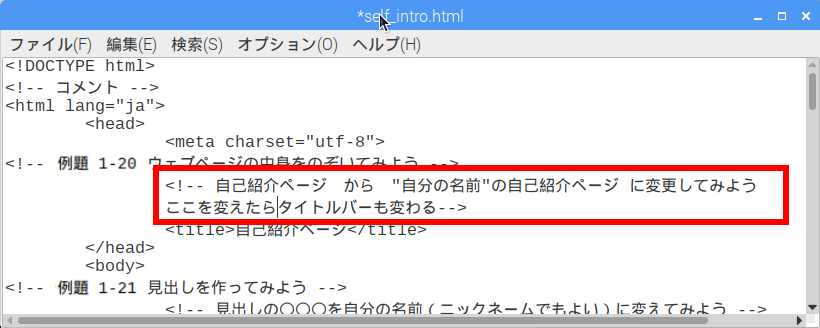
\includegraphics[width=0.85\textwidth]{textbook-img150.png}


\vfill
\clearpage
\begin{figure}[ht]
  \refstepcounter{Exercise}
  \subsection{\theExercise 見出しを作ってみよう}


  \centering
  \begin{minipage}{\textwidth}
    {\upshape
      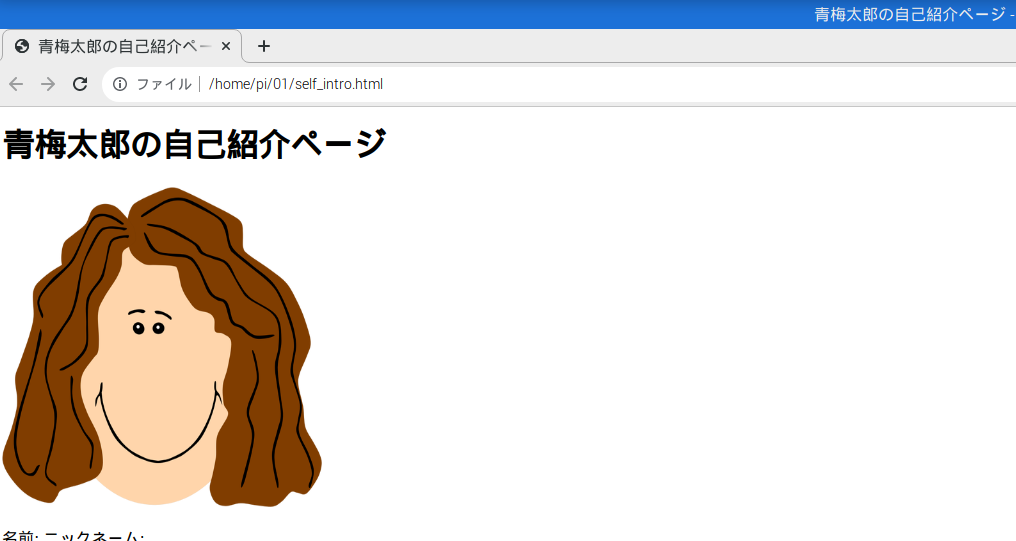
\includegraphics[width=0.7\textwidth]{textbook-img153.png}
      \newline
      \stepcounter{Figure}{\theFigure}: 見出しをつくってみよう}
  \end{minipage}


  \bigskip
  \flushleft

  \textbf{考え方}



  \begin{minipage}{\textwidth}
    \flushleft

    HTMLだけでなく見出しを作ることは読みやすい文書を作成するのに重要です。また、改行を適切に行うことも大切です。

    まずは、見出しを作ってみましょう。\textbf{〇〇〇の自己紹介ページ}を変更してみよう


    \bigskip

    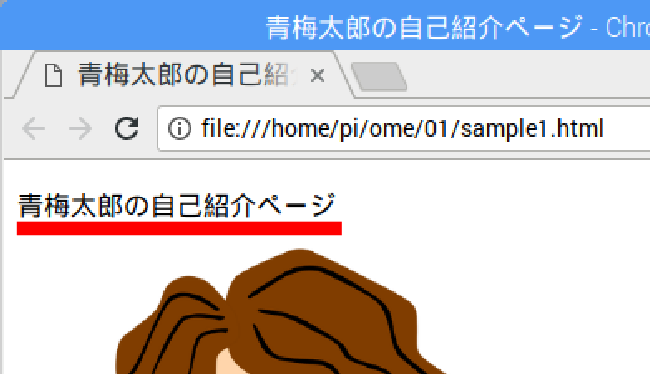
\includegraphics[width=0.7\textwidth]{textbook-img154.png}


    \bigskip

    テキストエディタで変更してみよう。変更したら保存してブラウザをリロードするのを忘れないようにしよう。


    \bigskip

    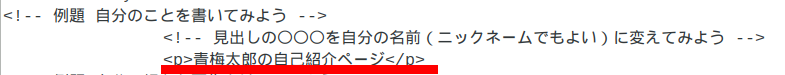
\includegraphics[width=0.9\textwidth]{textbook-img155.png}


    \bigskip


    見出しとしてはまだ文字が小さく目立たないですね。もっと大きくしてみましょう。




    \bigskip
  \end{minipage}

\end{figure}

\clearpage
\flushleft
\textbf{考え方(続き)}




次の行

{\textless}p{\textgreater}青梅太郎の自己紹介ページ{\textless}/p{\textgreater}

\bigskip

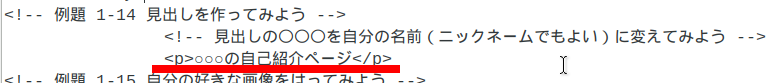
\includegraphics[width=0.9\textwidth]{textbook-img158.png}

から

{\textless}h1{\textgreater}青梅太郎の自己紹介ページ{\textless}/h1{\textgreater}

に変えてみましょう。保存してブラウザをリロードしてみてください。


\bigskip

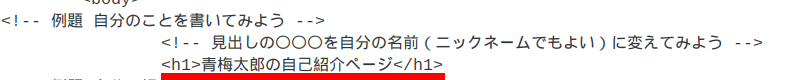
\includegraphics[width=0.9\textwidth]{textbook-img157.png}


\bigskip


\bigskip

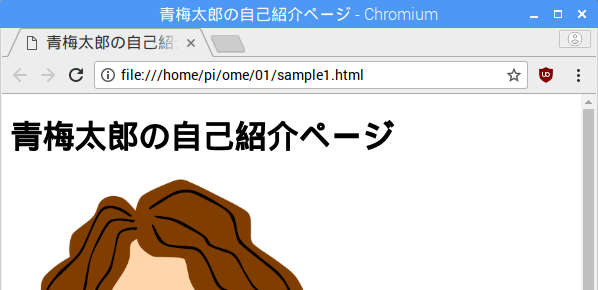
\includegraphics[width=0.4\textwidth]{textbook-img156.png}


今度は見出しらしく太文字で目立つようにになりましたね。




\bigskip

{\textless}p{\textgreater}青梅太郎の自己紹介ページ{\textless}/p{\textgreater} から

{\textless}h1{\textgreater}青梅太郎の自己紹介ページ{\textless}/h1{\textgreater} へ変更したら文字が太く大きくなりました。


\bigskip

{\textless}p{\textgreater}文字{\textless}/p{\textgreater}や{\textless}h1{\textgreater}文字{\textless}/h1{\textgreater}のようなものをそれぞれpタグ、h1タグといいます。\textbf{タグ}にはそれぞれ役割があります。タグの間に挟まれている文字に効果があります。

\begin{itemize}
  \item 文字の前にある{\textless}p{\textgreater}を\textbf{開始タグ}
  \item 文字の後にある{\textless}/p{\textgreater}を\textbf{終了タグ}
\end{itemize}

\textbf{タグには半角文字しかつかえません。}

\begin{itemize}
  \item pタグは、文章として表示をします。文章を書くときに使用します。

  \item h1タグは見出しとして表示をします。見出しを作るときに使用します。
\end{itemize}


\vfill

\refstepcounter{Question}\theQuestion\label{Q:hasAnswer04-2}

\begin{itemize}
  \item[]
    h1をh2、h3、h4、h5、h6にそれぞれ変えてみてどうなるか確かめてみましょう。
\end{itemize}

\bigskip

\clearpage\subsection{授業で使用するタグのいちらん}
{\small
  \begin{center}
    \tablefirsthead{}
    \tablehead{}
    \tabletail{}
    \tablelasttail{}
    \begin{supertabular}{|m{2.171cm}|m{4.1060004cm}|m{7.8930006cm}|m{2.037cm}|}
      \hline
      タグ名 &
      使用例 &
      効果 &
      例題番号\\\hline
      title &
      {\textless}title{\textgreater}タイトル{\textless}/title{\textgreater} &
      ブラウザのタイトルバーをタイトルに変更する
      &
      1-13\\\hline
      p &
      {\textless}p{\textgreater}文章{\textless}/p{\textgreater} &
      文章と表示する。改行なし &
      1-14\\\hline
      h1 &
      {\textless}h1{\textgreater}見出し1{\textless}/h1{\textgreater} &
      見出し1と表示する。普通の文字より大きい
      &
      1-14\\\hline
      img &
      {\textless}img src=”img.png”{\textgreater} &
      src=””で指定された画像ファイルを表示する
      &
      1-15\\\hline
      br &
      {\textless}br{\textgreater} &
      改行をする &
      1-16\\\hline
      ol &
      {\textless}ol{\textgreater}

      \ \ {\textless}li{\textgreater}1位{\textless}/li{\textgreater}

      {\textless}/ol{\textgreater} &
      liタグと合わせて使用する。順序付きのリストを作る。順序はliタグの順番通りにつく
      &
      1-17\\\hline
      Ul &
      {\textless}ul{\textgreater}

      \ \ {\textless}li{\textgreater}1位{\textless}/li{\textgreater}

      {\textless}/ul{\textgreater} &
      順序なし。${\bullet}で始まるリストを作成。$
      &
      1-20\\\hline
      i &
      {\textless}i{\textgreater}イタリック{\textless}/i{\textgreater} &
      斜めの文字を表示 &
      1-18\\\hline
      u &
      {\textless}u{\textgreater}アンダーライン{\textless}/u{\textgreater} &
      下線つきの文字を表示 &
      1-18\\\hline
      strong &
      {\textless}strong{\textgreater}

      目立つ文字

      {\textless}/strong{\textgreater} &
      文字を目立たせる &
      1-18\\\hline
      font  &
      {\textless}font color=”\#019a66”{\textgreater}

      \ \ 色付き文字

      {\textless}/font{\textgreater} &
      color=””で指定した色で文字を表示。 &
      1-18\\\hline
      font &
      {\textless}font size=”1”{\textgreater}

      大きさを変える

      {\textless}/font{\textgreater} &
      size=””で指定した文字の大きさで表示 &
      1-18\\\hline
      table &
      {\textless}table{\textgreater}

      ~

      {\textless}/table{\textgreater} &
      表を作成するときに使用する。caption, tr, th,
      tdタグといっしょに使用する。 &
      1-19\\\hline
      caption &
      {\textless}caption{\textgreater}表題{\textless}/caption{\textgreater} &
      表のタイトルを表示 &
      1-19\\\hline
      tr &
      {\textless}tr{\textgreater}{\textless}/tr{\textgreater} &
      表の行を作る。th,
      tdタグといっしょに使用する。 &
      1-19\\\hline
      th &
      {\textless}th{\textgreater}列のタイトル{\textless}/th{\textgreater} &
      表の列のタイトルを表示する &
      1-19\\\hline
      td &
      {\textless}td{\textgreater}列のデータ{\textless}/td{\textgreater} &
      表の列のデータを表示 &
      1-19\\\hline
      a &
      {\textless}a href=”google.com”{\textgreater}

      \ \ google

        {\textless}/a{\textgreater} &
      クリックすると登録していたホームページに移動する文字を表示
      &
      1-20\\\hline
    \end{supertabular}
  \end{center}
}

\bigskip
ホームページを作るときには、これらのタグをたくさん使用します。使い方を例題とともに学んでいきましょう。


\clearpage


{\centering\bfseries
  タグは半角文字で入力しなければなりません。
  \par}

{\centering\bfseries
  HTMLファイルでタグを入力する際は
  \par}

{\centering\bfseries
  常に右上のアイコンがキーボードになっていることを確認してください。
  \par}

\centering
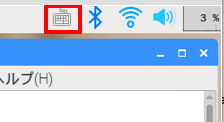
\includegraphics[width=0.6\textwidth]{textbook-img159.png}





\bigskip

\bigskip

\bigskip

\bigskip


{\centering\bfseries
  このアイコンのときは全角入力モードだから
  \par}

\centering
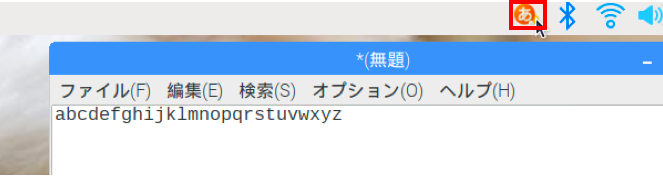
\includegraphics[width=0.6\textwidth]{textbook-img160.png}


\bigskip


\bigskip

{\centering\bfseries
  タグを打つときはCtrl +
  スペースキーを押して半角入力モード
  \par}

{\centering\bfseries
  (キーボードのアイコン)にしよう
  \par}

\clearpage
%\begin{figure}[ht]
\flushleft
\refstepcounter{Exercise}
\subsection{\theExercise 自分の好きな画像をはってみよう}
\addtocounter{Exercise}{-1}\refstepcounter{Exercise}\label{E:embImginHTML}
自分のお気に入りの画像を紹介してみよう。

\centering
\begin{minipage}{6.738cm}
  {\upshape
    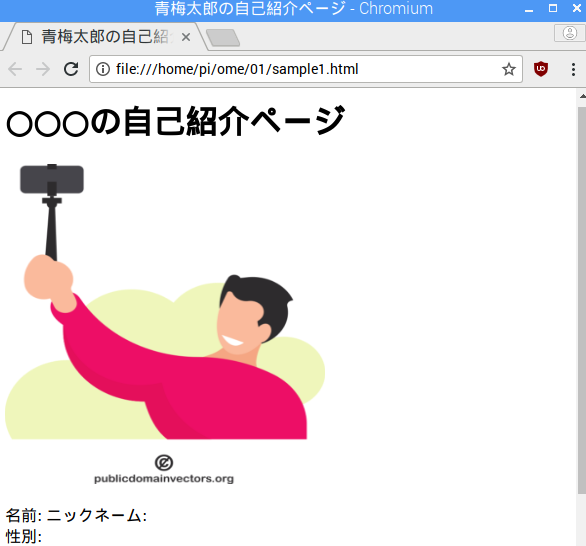
\includegraphics[width=7.071cm,height=6.048cm]{textbook-img161.png}
    \newline
    \stepcounter{Figure}{\theFigure}: 顔写真}
\end{minipage}

\flushleft
\textbf{考え方}


いま、髪の長い人の写真が表示されているところがあります。このように自分の好きな画像を表示させることができます。試しに、ウェブカメラでとった自分の顔に変えてみましょう。

まずは、画像をコピーします。


\bigskip

\begin{minipage}{0.45\linewidth}
  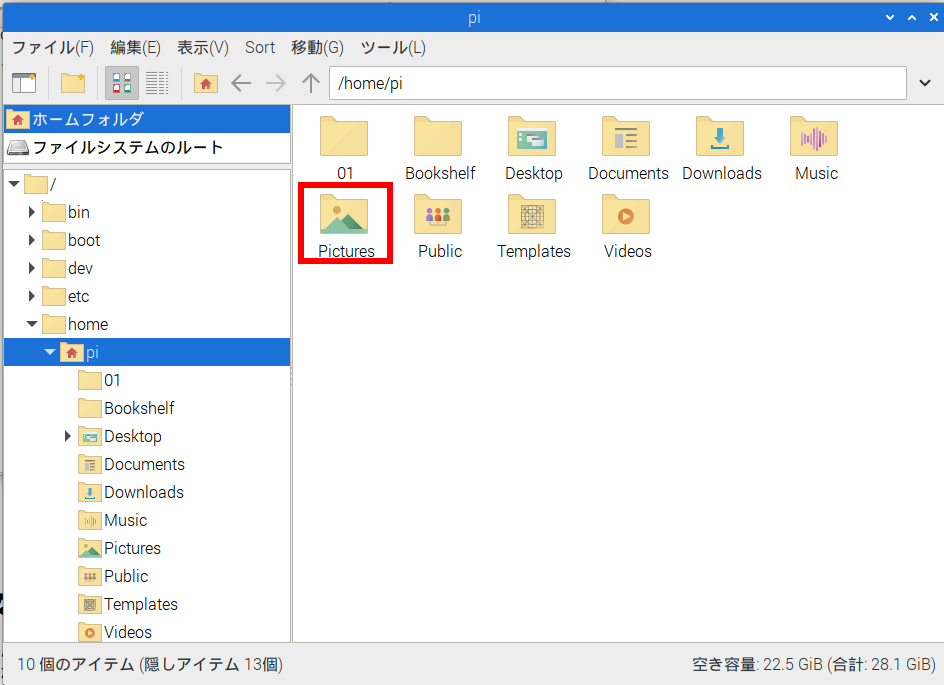
\includegraphics[width=\linewidth]{textbook-img164.png}
  \newline
  1 Picturesをダブルクリック
\end{minipage}
\hspace{10mm}
\begin{minipage}{0.45\linewidth}
  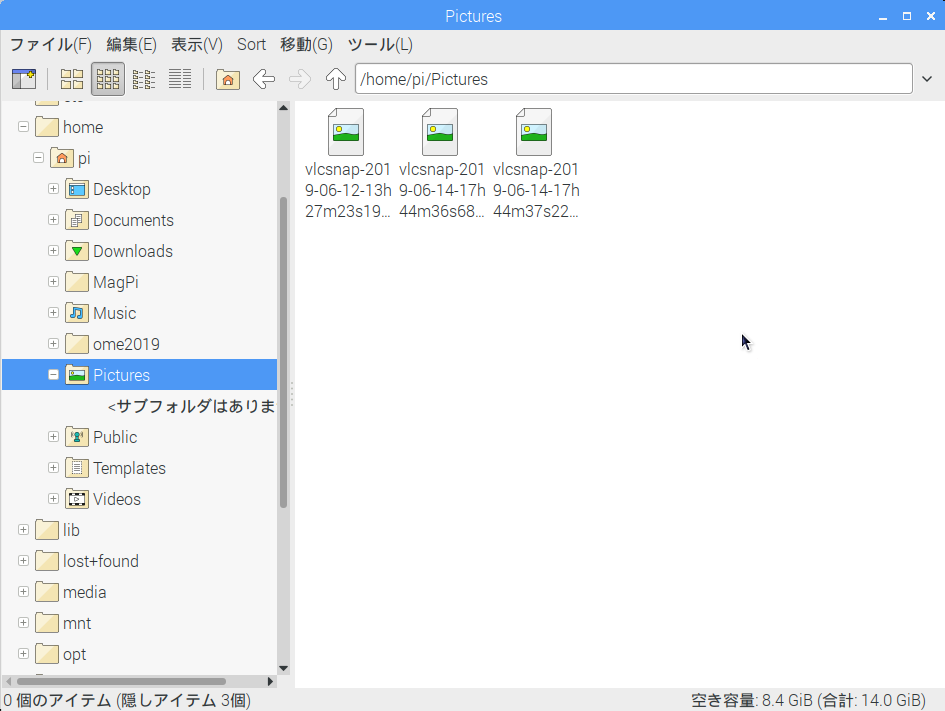
\includegraphics[width=\linewidth]{textbook-img162.png}
  \newline
  2 使いたい画像を右クリック
\end{minipage}

\bigskip

\begin{minipage}{0.45\linewidth}
  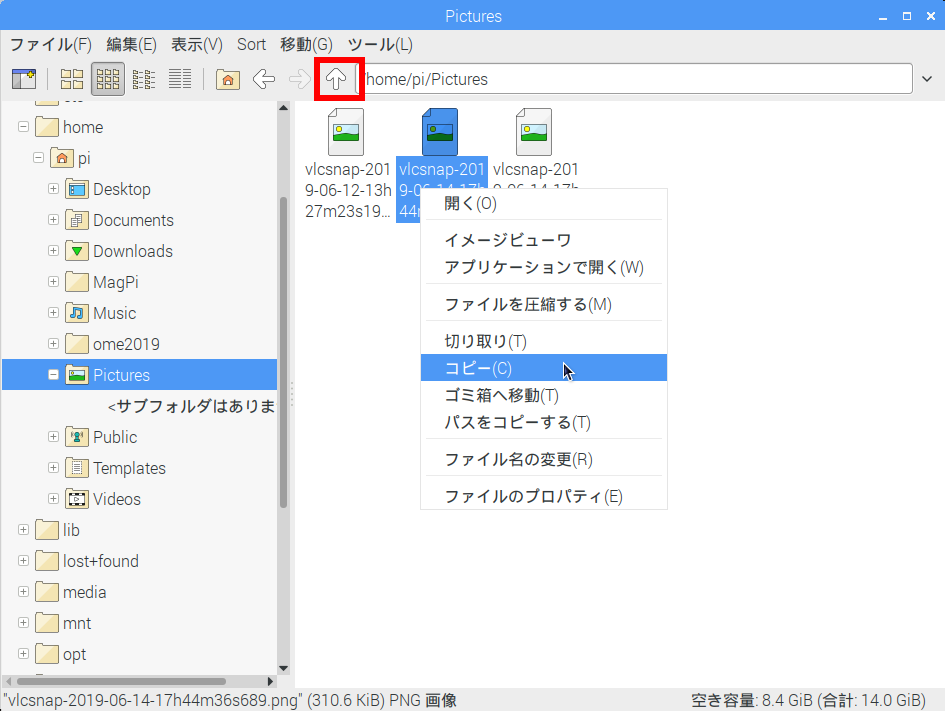
\includegraphics[width=\linewidth]{textbook-img163.png}
  \newline
  3
  コピーを選択・赤枠の上矢印をクリック
\end{minipage}
\hspace{10mm}
\begin{minipage}{0.45\linewidth}
  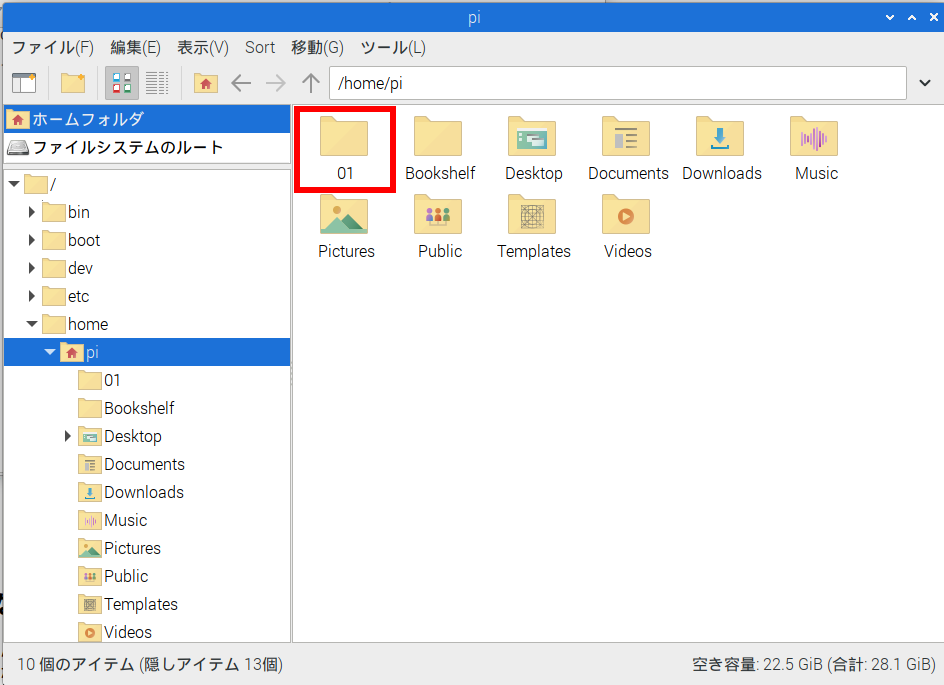
\includegraphics[width=\linewidth]{textbook-img167.png}
  \newline
  4 01をダブルクリック
\end{minipage}

\clearpage
\flushleft

\textbf{考え方}


\bigskip


\bigskip


\bigskip

\centering
\begin{minipage}{0.45\linewidth}
  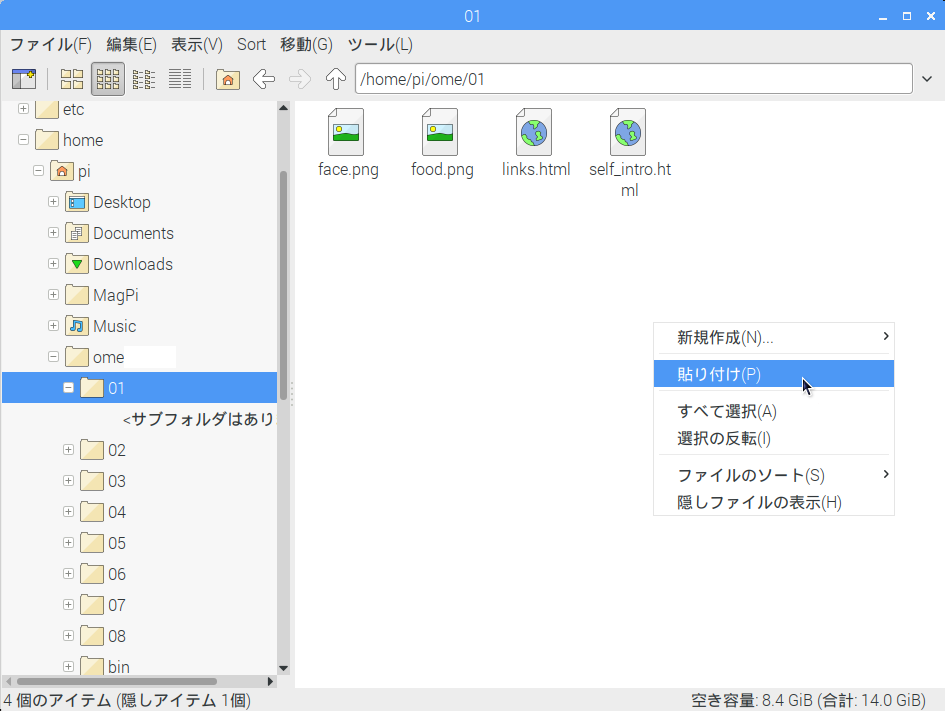
\includegraphics[width=\linewidth]{textbook-img168.png}\\
  5 右クリックして貼り付けを選択します
\end{minipage}
\hfill
\vspace{20pt}
\begin{minipage}{0.45\linewidth}
  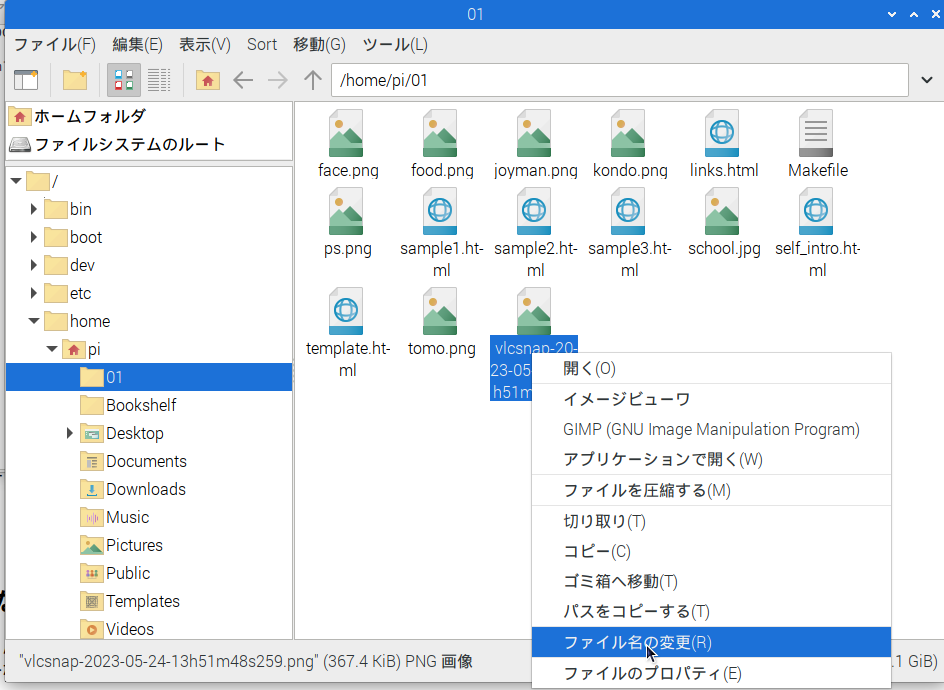
\includegraphics[width=\linewidth]{textbook-img169.png}\\
  6 貼り付けたファイルを右クリックして、「ファイル名の変更」をします
\end{minipage}
\begin{minipage}{0.45\linewidth}
  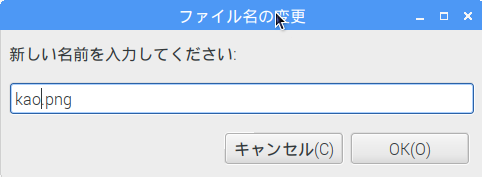
\includegraphics[width=\linewidth]{textbook-img166.png}\\
  7 今回は「kao.png」と変更します
\end{minipage}
\hfill
\vspace{20pt}
\begin{minipage}{0.45\linewidth}
  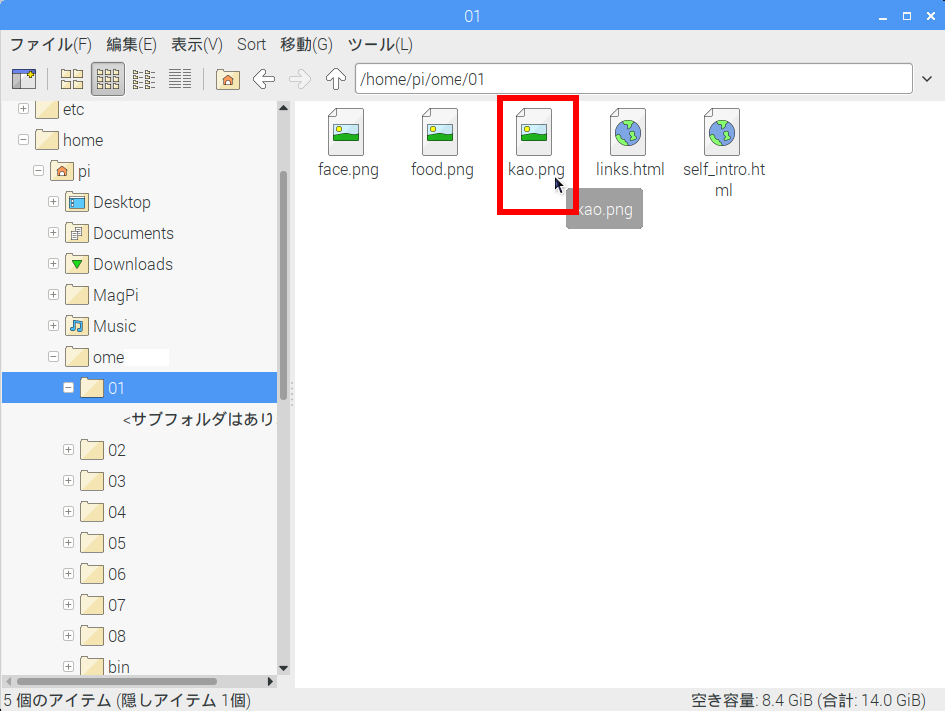
\includegraphics[width=\linewidth]{textbook-img170.png}\\
  8 これで画像のコピーは完了です。次はhtmlを編集し、自己紹介ページに表示しましょう
\end{minipage}

\clearpage
\flushleft
\textbf{考え方}\ \


赤色で線を引いているところで画像を表示しています。\\
\textbf{{\textless}img href=”face.png” width=”320” height=”320”{\textgreater}}
\textbf{href=””で画像のファイルを指定しています。}\\
\textbf{“face.png”}からコピーしたファイル\textbf{(“kao.png”)}へ変更してみましょう。

\begin{minipage}{\textwidth}
  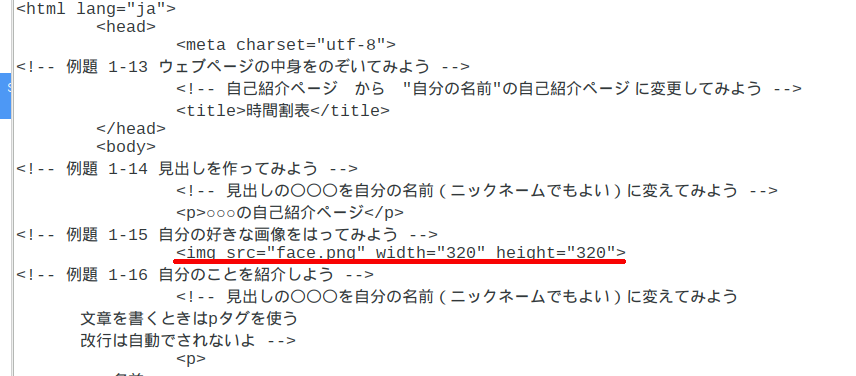
\includegraphics[width=0.6\textwidth]{textbook-img171.png}
  \newline
  変更して、保存しリロードするととった写真が表示されます。
\end{minipage}

\flushleft
\textbf{答え}

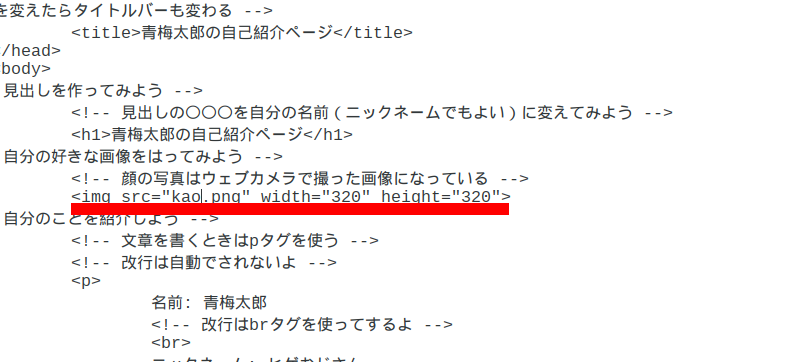
\includegraphics[width=0.6\textwidth]{textbook-img172.png}



\refstepcounter{Question}\theQuestion

スパゲッティの画像をウェブカメラでとった画像(教室の風景など)に変更しよう

ヒント

%\liststyleLxviii
\begin{enumerate}
  \item
        画像を01フォルダの中にコピーして名前を変更しよう。
  \item
        imgタグをコピーした画像を表示するように変更しよう
\end{enumerate}
\refstepcounter{Question}\theQuestion\label{Q:hasAnswer04-3}

width,
heightを変更して画像の大きさを変えてみましょう

ヒント

%\liststyleLxix
\begin{itemize}
  \item
        widthは横幅、heightはたて幅です。数字を変えて見ましょう。
\end{itemize}


\clearpage
\refstepcounter{Exercise}
\subsection{\theExercise 自分のことを紹介しよう}
\centering
\begin{minipage}{\textwidth}
  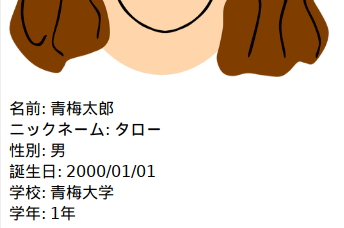
\includegraphics[width=0.5\textwidth]{textbook-img173.png}
  \newline
  \stepcounter{Figure}{\theFigure}: 自分のことを紹介しよう
\end{minipage}

\bigskip

\flushleft

\textbf{考え方}


\bigskip

まずは今回変更する場所をブラウザで見てみましょう。

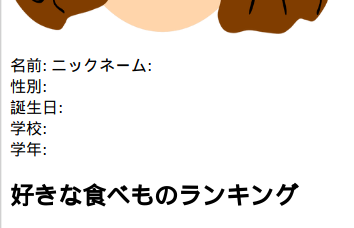
\includegraphics[width=0.5\textwidth]{textbook-img175.png}

\bigskip

\flushleft
名前とニックネームが同じ行になっていて、見づらいですね。まずは、改行の仕方を学びましょう。テキストエディタへ戻ってください。文章中で改行をするには\\
{\textless}br{\textgreater} \ \ \ \ \ \\
タグを使います。このタグには終了タグがありません。赤線を引いてある下に{\textless}br{\textgreater}タグをいれて改行できているか確かめてみましょう。


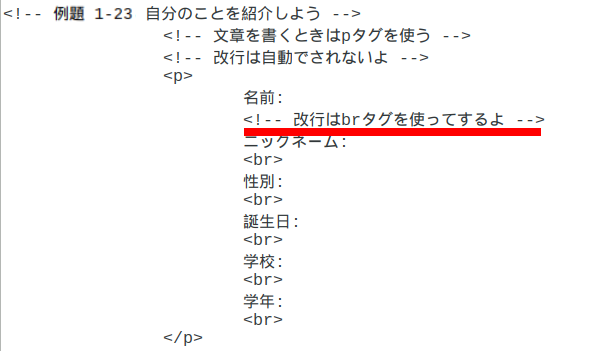
\includegraphics[width=0.5\textwidth]{textbook-img174.png}

\clearpage
\flushleft

\textbf{考え方(続き)}


これで見やすくなりましたね。

\bigskip


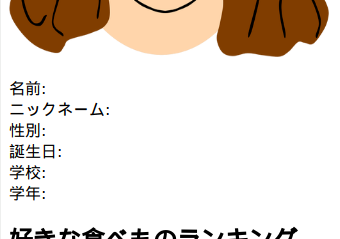
\includegraphics[width=0.5\textwidth]{textbook-img176.png}

\bigskip

次は自分のことを紹介しよう。\\
名前、性別、誕生日、学校、学年\\
を追加してみよう。



\bigskip

\bigskip


\textbf{答え}


\bigskip

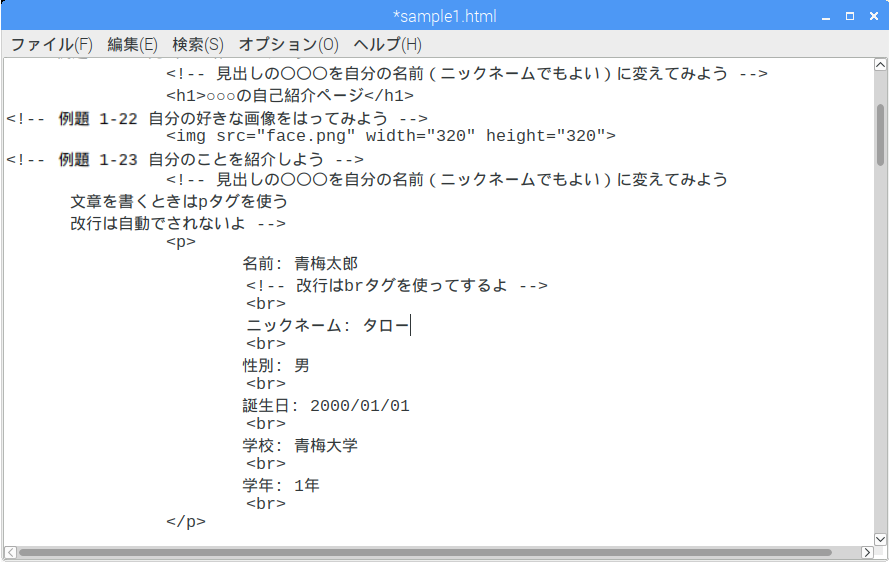
\includegraphics[width=0.5\textwidth]{textbook-img177.png}



\bigskip

\bigskip



ブラウザの画面

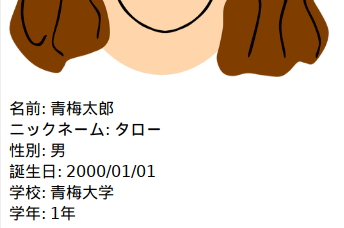
\includegraphics[width=0.5\textwidth]{textbook-img173.png}



\clearpage
\refstepcounter{Question}\theQuestion\label{Q:hasAnswer04-4}

他にも紹介項目を追加してみましょう

%\liststyleLxx
\begin{itemize}
  \item ヒント : しゅみ、すきなもの
\end{itemize}
\refstepcounter{Question}\theQuestion\label{Q:hasAnswer04-5}

顔写真の変更

ヒント

%\liststyleLxxi
\begin{enumerate}
  \item
        01フォルダに画像をコピーしよう。
  \item とった画像はPicturesフォルダにあるよ。
  \item 画像の名前を変えよう。
  \item
        imgタグを変えて、表示させたい画像のファイル名にしよう。
\end{enumerate}

\bigskip


\bigskip

\clearpage
\refstepcounter{Exercise}
\subsection{\theExercise ランキングを作ろう}
自分の好きなことを紹介するためにランキングトップ3を作ってみましょう。見出しの変更とランキングに一つ追加する必要があります。



\bigskip


\begin{minipage}{\textwidth}
  {\upshape
    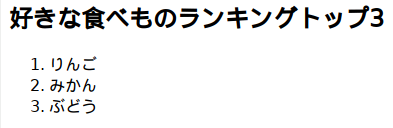
\includegraphics[width=0.65\textwidth]{textbook-img178.png}
    \newline
    \stepcounter{Figure}{\theFigure}:
    好きなたべものランキングトップ3を作ろう}
\end{minipage}


\bigskip


\bigskip

\textbf{考え方}



\bigskip



好きなたべものランキングトップ3を作ってみましょう。まずは、ブラウザで確認してみましょう。


\bigskip

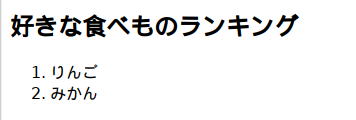
\includegraphics[width=0.65\textwidth]{textbook-img179.png}

\bigskip

まずは、見出しを変更してみましょう。\\
\textbf{好きなたべものランキングトップ3}\\
に変えてください。


\bigskip

次にランキングの作り方を説明します。\\
ランキングを作るにはリストを使います。テキストエディタを見てみましょう。

\centering
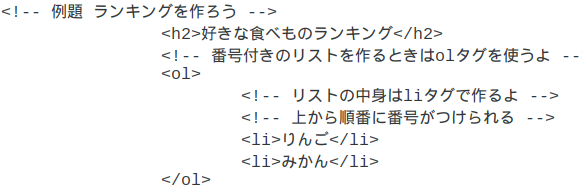
\includegraphics[width=0.6\textwidth]{textbook-img180.png}

\clearpage
\flushleft
\textbf{考え方(続き)}


\bigskip


ランキングの\textbf{りんご}は青色で線が引かれている行で表示をしています。


\bigskip


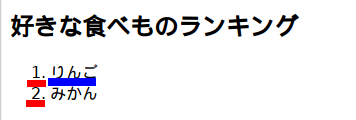
\includegraphics[width=0.65\textwidth]{textbook-img182.png}


\bigskip


%[Warning: Image ignored] % Unhandled or unsupported graphics:
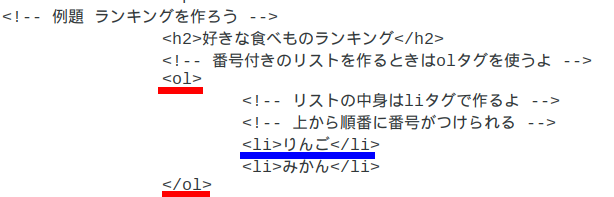
\includegraphics[width=0.6\textwidth]{textbook-img181.png}


青色で線が引かれている行の\\
{\textless}li{\textgreater}りんご{\textless}/li{\textgreater}\\
りんごを表示しています。\\
順位は赤で線が引かれている\\
{\textless}ol{\textgreater}\\
{\textless}/ol{\textgreater}\\
で表示をしています。リストを使ってランキングを作るには、\\
{\textless}ol{\textgreater}\\
\ \ {\textless}li{\textgreater}りんご{\textless}/li{\textgreater}\\
{\textless}/ol{\textgreater}\\
のように順位をつけるolタグの中でliタグを使い文字を囲みます。\\
練習として\textbf{ぶどう}をランキングの一番下に追加しましょう。\\


\bigskip


\includegraphics[width=0.9\textwidth]{textbook-img183.png}


\bigskip


保存してブラウザをリロードすると\textbf{ぶどう}が一番下に表示されました。書いた順番に順位がつきます。

りんご、みかん、ぶどうを実際に好きなたべものに変えてみてください。


\bigskip
\clearpage
\textbf{答え}


\bigskip



\includegraphics[width=0.9\textwidth]{textbook-img184.png}


\bigskip


\bigskip


\bigskip


\refstepcounter{Question}\theQuestion\label{Q:hasAnswer04-6}

ランキングを追加してみましょう

ヒント

%\liststyleLxxii
\begin{itemize}
  \item
        好きなお菓子ランキング、好きなYouTuberランキング
\end{itemize}


\bigskip

\bigskip

\refstepcounter{Question}\theQuestion\label{Q:hasAnswer04-7}

ヒント

%\liststyleLxxiii
\begin{itemize}
  \item
        {\textless}ol{\textgreater}{\textless}/ol{\textgreater}の代わりに{\textless}ul{\textgreater}{\textless}/ul{\textgreater}を使って、どうなるか確認してみましょう
\end{itemize}



\bigskip

\clearpage
\refstepcounter{Exercise}
\subsection{\theExercise 日記を書いてみよう}
日記を書いてみよう。教室でやっていることを紹介してみよう。

\centering
\begin{minipage}{6.32cm}
  {\upshape
    \includegraphics[width=0.45\textwidth]{textbook-img185.png}
    \newline
    \stepcounter{Figure}{\theFigure}: 日記を書いてみよう}
\end{minipage}

\bigskip

\flushleft
\textbf{考え方}



文章を書くときは{\textless}p{\textgreater}{\textless}/p{\textgreater}を使うと習いました。

文字の太さ、色を変えたり、アンダーライン、ななめ文字にすることもできます。

\centering
\includegraphics[width=14.284cm]{textbook-img186.png}

\bigskip

\flushleft

イタリックはななめの文字です。イタリックという文字が少しななめになっているのを確認してみましょう\\
{\textless}i{\textgreater}イタリック{\textless}/i{\textgreater}\\

\bigskip

アンダーラインは文字の下に線を引きます。\\
{\textless}u{\textgreater}アンダーライン{\textless}/u{\textgreater}\\

\bigskip

太文字は文字を太くします\\
{\textless}strong{\textgreater}\textbf{あいうえお}{\textless}/strong{\textgreater}


\bigskip
色付きの文字は
\textbf{{\textless}font color=”\#RRGGBB”{\textgreater}色文字{\textless}/font{\textgreater}}
として光の三原色を用いて色を指定します。\\
\textbf{RR}は赤の強さ\\
\textbf{GG}は緑の強さ\\
\textbf{BB}は青の強さを、
それぞれ00からFFの16進数で指定します。
例えば、赤は"\#FF0000"、緑は"\#00FF00"、青は"\#0000FF"、白は"\#FFFFFF"、黒は"\#000000"

\bigskip
\textbf{16進数は、0から9の次に、A,B,C,D,E,Fを用いて、
  1桁を16個の数値で表します。}

\bigskip



\clearpage
\textbf{考え方(続き)}



\textbf{授業で使用したホームページ\url{links.html}の2番目}を開いて見てください。
2番を開くと地下鉄で使っている色の見本が出てきます。
銀座線オレンジは\textbf{\#f39700}となっているので、
上のcolorの値を”\#f39700”とします。
このように数値によって表示する色を選びます。



\bigskip

\includegraphics[width=\textwidth]{textbook-img187.png}

文字の大きさを変えるときは

\textbf{{\textless}font size=”1”{\textgreater}文字の大きさ{\textless}/font{\textgreater}}

\textbf{size=”1”}で文字の大きさを変えられます。1を他の数字に変えてみてください。

このように文字のとくちょうを変えることができます。


\bigskip

これらのタグを使って日記を書いてみよう。

下の日記を参考にしてみよう


\bigskip

\includegraphics[width=8.779cm]{textbook-img185.png}

\clearpage
\textbf{答え}



\includegraphics[width=\textwidth]{textbook-img188.png}

\refstepcounter{Question}\theQuestion\label{Q:hasAnswer04-8}
\textbf{{\textless}hr{\textgreater}}タグを使うと横線を引くことができます。日記の一番下に横線を引いてみよう。

ヒント

%\liststyleLxxiv
\begin{itemize}
  \item
        終了タグはhrタグにありません。{\textless}hr{\textgreater}と書いたところに横線が表示されます。
\end{itemize}
\refstepcounter{Question}\theQuestion\label{Q:hasAnswer04-9}

日記をもう一つ追加してみよう

ヒント

%\liststyleLxxv
\begin{itemize}
  \item
        タイトル、日付、本文を順番に書いてみよう。
\end{itemize}
\clearpage
\refstepcounter{Exercise}
\subsection{\theExercise グループのメンバー表を作ろう}
グループの友だちのことを表にまとめてみよう。

\centering
\begin{minipage}{\textwidth}
  {\upshape
    \includegraphics[width=0.5\textwidth]{textbook-img189.png}
    \newline
    \stepcounter{Figure}{\theFigure}: グループメンバーの表}
\end{minipage}

\bigskip

\flushleft
\textbf{考え方}



表を作るには

{\textless}table{\textgreater}{\textless}/table{\textgreater}

を使います。

まずは、表に題名をつけます。captionタグを使います。

青色の線を見てください。

\textbf{{\textless}caption{\textgreater}みんなの紹介{\textless}/caption{\textgreater}}

の行が表の題名として表示されています。



\bigskip

\includegraphics[width=13.462cm]{textbook-img190.png}


\bigskip

その次に、列の見出しをつけます。緑色で囲われているところを見てください。\\
表の1行目に名前、学校、学年という項目があります。行は横方向です。\\
行を作るにはtrタグを使います。\\
行の見出しはthタグを使います。\\


\bigskip

{\textless}tr{\textgreater}\\
\ \ {\textless}th{\textgreater}名前{\textless}/th{\textgreater}\\
{\textless}/tr{\textgreater}\\

\bigskip

\clearpage
\textbf{考え方(続き)}



\bigskip

\bigskip


\centering
\includegraphics[width=\textwidth]{textbook-img191.png}

\flushleft

\bigskip

表の1行目にある見出しの次は実際の情報がきます。2行目は青色で囲われているところです。

0くんのことが書いてあります。行を作るにはtrタグを使います。

見出しではthタグを使いました。見出しでない行ではtdタグを使って列の情報を表示させます。

{\textless}tr{\textgreater}

\ \ {\textless}td{\textgreater}0くん{\textless}/td{\textgreater}

\ \ {\textless}td{\textgreater}c中学校{\textless}/td{\textgreater}

\ \ {\textless}td{\textgreater}2年生{\textless}/td{\textgreater}

{\textless}/tr{\textgreater}

一個目のtdタグは一個目のthタグに対応しています。つまり、一個目のthタグの\textbf{名前}は一個目のtdタグの0くんに対応しています。


\bigskip


\bigskip

グループのメンバーの友だちの名前、学校、学年を聞いてtdタグを書き換えてみよう。


\bigskip


\bigskip



\bigskip

\clearpage
\textbf{答え}




\bigskip


\bigskip


\bigskip
\includegraphics[width=\textwidth]{textbook-img192.png}




\bigskip

\bigskip

\bigskip

\refstepcounter{Question}\theQuestion

表にクラスを追加してみよう。

ヒント

%\liststyleLxxvi
\begin{enumerate}
  \item クラスを見出しに追加してみよう
  \item
        みんなのクラスを聞いて、追加してみよう
\end{enumerate}
\refstepcounter{Question}\theQuestion

TAのことを追加してみよう

%\liststyleLxxvii
\begin{itemize}
  \item
        TAの先生に名前、学校、学年、クラスを聞いて表に追加してみよう
\end{itemize}

\bigskip

\clearpage

\refstepcounter{Exercise}
\subsection{\theExercise 自分の好きなホームページを紹介しよう}
自分のお気に入りのサイトを自分のホームページで紹介しよう。



\centering
\begin{minipage}{\textwidth}
  {\upshape
    \centering
    \includegraphics[width=0.4\textwidth]{textbook-img193.png}
    \newline
    \stepcounter{Figure}{\theFigure}:
    自分の好きなホームページを紹介しよう}
\end{minipage}



\bigskip

\flushleft

\textbf{考え方}



まずはブラウザを見てみましょう。赤線で線を引いてあるところはリンクといい、クリックすると登録されているホームページへ移動します。試しにgoogleをクリックして見てください。


\bigskip

\centering
\includegraphics[width=0.22\textwidth]{textbook-img194.png}


\flushleft

\bigskip

クリックをするとブラウザで開いているページがリンクされているページへ移動します。

赤色で囲われているところがホームページの住所にあたる部分です。この部分をリンクとして登録します。青色で囲われている矢印を押すと前のページへ戻ります。自分のページへ戻りましょう。



\bigskip

\centering
\includegraphics[width=0.22\textwidth]{textbook-img195.png}

\bigskip

\flushleft
次は、タイピングゲームをクリックして見てください。今回はページは移動しません。まだタイピングゲームのホームページを登録していないからです。


\clearpage
\textbf{考え方(続き)}



試しに少し前に遊んだタイピングゲームを自分のページから移動できるようにしておきましょう。まずは、タイピングゲームのページを開いてください。開けたら赤線を引いたホームページの住所にあたる部分をクリックします。その後、右クリックをして\textbf{すべてを選択(A)}をクリックします。


\bigskip

\centering
\includegraphics[width=0.3\textwidth]{textbook-img196.png}

\flushleft

その後、赤線を引いてある住所にあたる部分が青くなります。そしたらまた右クリックをして

\textbf{コピー(C)}をクリックします。住所にあたる部分をコピーしました。

\centering
\includegraphics[width=0.3\textwidth]{textbook-img197.png}

\bigskip
\flushleft

次は、テキストエディタを開きます。

\centering
\includegraphics[width=\textwidth]{textbook-img198.png}

\bigskip
\flushleft

リンクは赤線を引いてあるように

{\textless}a
href=”ホームページの住所”{\textgreater}タイピングゲーム{\textless}/a{\textgreater}

と書きます。今の状態では\textbf{ホームページの住所}はくうらんです。

くうらんになっているところを左クリックしてから右クリックします。そこで\textbf{貼り付け(P)}をします。





\centering
\includegraphics[width=0.25\textwidth]{textbook-img199.png}

\clearpage
\flushleft
\textbf{考え方(続き)}


\bigskip

\centering
\includegraphics[width=\textwidth]{textbook-img200.png}

\bigskip
\flushleft

これでタイピングゲームのホームページの住所を登録できました。保存してブラウザをリロードしてください。タイピングゲームをクリックするとタイピングゲームのホームページへ移動するようになりました。


\bigskip
\centering
\includegraphics[width=0.25\textwidth]{textbook-img201.png}


\flushleft
このようにリンクを追加します。自分の好きなホームページをリンクとして表示してみてください。

ちなみに、先程のランキングを作るときにはolタグを使って順序をつけました。今回は順序ではなく${\bullet}を使っています。そのため青線で引いたように${\textless}ul{\textgreater}{\textless}/ul{\textgreater}を代わりに使います。

ulタグをolタグに変えれば順序をつけることができます。


\bigskip

\textbf{答え}

\centering
\includegraphics[width=0.9\textwidth]{textbook-img202.png}

\flushleft
\refstepcounter{Question}\theQuestion\label{Q:hasAnswer04-10}


ホームページのランキングを作ってみよう。

ヒント

%\liststyleLxxviii
\begin{enumerate}
  \item リストに順序をつけよう
  \item リストの項目をaタグにしよう
\end{enumerate}

\clearpage
\refstepcounter{Exercise}
\subsection{\theExercise 教室の使うものリストを作ろう}
教室に使うものリストを作ろう

\bigskip
\centering
\begin{minipage}{5.937cm}
  {\upshape
    \includegraphics[width=5.937cm]{textbook-img203.png}
    \newline
    \stepcounter{Figure}{\theFigure}: 教室で使うものリスト}
\end{minipage}

\bigskip
\flushleft

\textbf{考え方}



リストを作るのには

{\textless}ul{\textgreater}

\ \ {\textless}li{\textgreater}リスト項目1{\textless}/li{\textgreater}

{\textless}/ul{\textgreater}

のように書くと習いました。リストの中にリストを入れることもできます。

テキストエディタを見てください

\bigskip

\centering
\includegraphics[width=0.9\textwidth]{textbook-img204.png}

\bigskip
\flushleft

赤線が引かれているulタグの中に青色で囲われているulタグがありますね。ブラウザで見てみると、

${\bullet}持ち帰るもの$

\ \ ◯ラズベリーパイ

のようになっています。このように、ulタグの中でulタグを使うと、リストの中でリストをかけるようになります。

ラズベリーパイの下に項目を追加してみましょう。


\bigskip


\clearpage\flushleft
\textbf{答え}


\bigskip

\centering
\begin{minipage}{0.45\linewidth}
  \includegraphics[width=\linewidth]{textbook-img1043.png}
\end{minipage}
\hfill
\vspace{20pt}
\begin{minipage}{0.45\linewidth}
  \includegraphics[width=\linewidth]{textbook-img1044.png}
\end{minipage}

\bigskip
\flushleft

\refstepcounter{Question}\theQuestion\label{Q:hasAnswer04-11}

持ち物の画像をとって、項目の下に貼ろう

ヒント

%\liststyleLxxix
\begin{enumerate}
  \item
        ウェブカメラで持ち物の画像をとってみよう
  \item
        01フォルダの中に画像をコピーしよう
  \item 画像の名前を変更しよう
  \item
        imgタグをliタグの下に追加して、画像を表示させよう。
\end{enumerate}

\bigskip


\clearpage
\end{document}
